\section{Experimental Setup}
\label{sec:setup}

\subsection{Benchmark: SynthShapes-32}
Directly measuring \emph{localisation} quality of an explanation requires knowing
where the discriminative object actually is---information that natural-image
benchmarks such as CIFAR-10 do not provide at the pixel level. We therefore
construct \textbf{SynthShapes-32}, a controlled $32\times32$ RGB benchmark of six
shape classes (\textsc{disk, square, triangle, cross, ring, bar}) rendered at a
random location on a textured, low-frequency background with additive Gaussian
sensor noise ($\sigma=0.12$). Crucially, the binary object mask $\bm M$ is known
by construction, enabling the $\mathrm{IoU}_{\mathrm{GT}}$ and pointing-game
metrics of Section~\ref{sec:prelim}. Class colours overlap so that the task is
non-trivial (shape, not colour, is decisive). We generate $3000$ training and
$1000$ test images with disjoint seeds. Fig.~\ref{fig:dataset} shows samples with
their masks. This design mirrors the statistical regime of small natural-image
benchmarks while giving the ground truth needed for a rigorous fidelity study;
the same protocol transfers unchanged to CIFAR-scale data where masks are
unavailable and only model-vs-model fidelity can be evaluated.

\begin{figure}[!t]
\centering
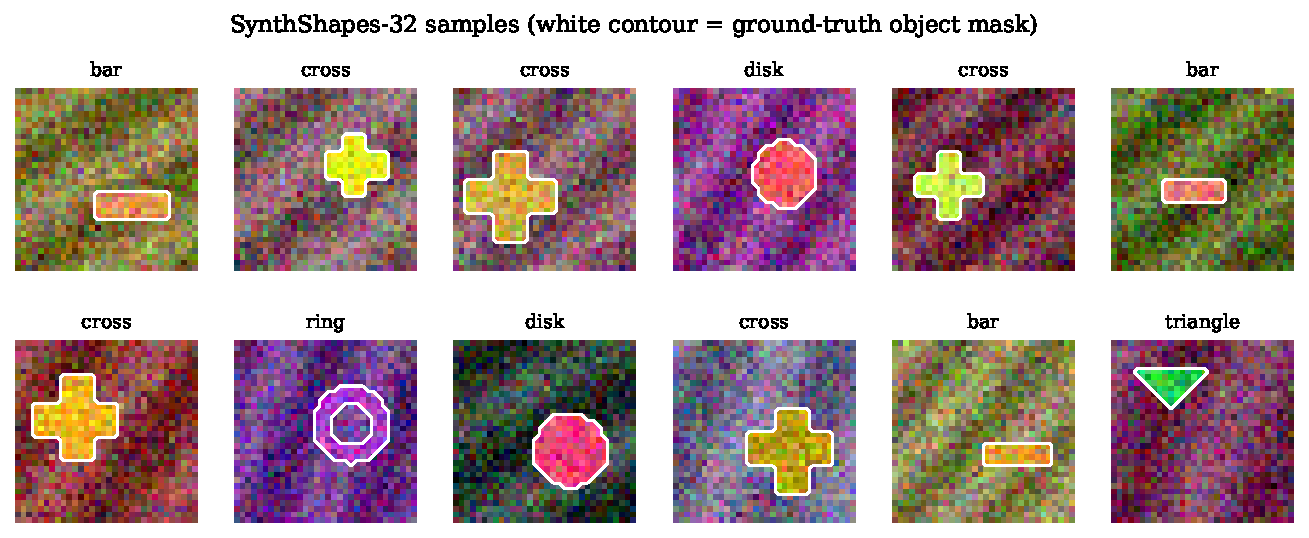
\includegraphics[width=\columnwidth]{figs/dataset.pdf}
\caption{Samples from the SynthShapes-32 benchmark. The white contour marks the
ground-truth object mask $\bm M$ used to evaluate explanation localisation.}
\label{fig:dataset}
\end{figure}

\subsection{Model and Training}
The classifier is a compact residual CNN \cite{he2016resnet} whose global-average-pooling (GAP) head
makes the final residual block the natural Grad-CAM target. The full training
recipe is:
\begin{itemize}
\item \textbf{Architecture:} $3\times3$ stem $\to$ three residual stages of width
$(16,32,64)$ $\to$ GAP $\to$ linear head ($77{,}782$ parameters).
\item \textbf{Optimiser:} Adam, learning rate $10^{-3}$, weight decay
$5\times10^{-4}$, cosine schedule.
\item \textbf{Schedule:} $14$ epochs; final test accuracy $98.5\%$.
\item \textbf{Hardware:} a single CPU core with ${<}4$\,GB RAM---matching the
constrained devices that motivate compression; the identical pipeline also runs
unmodified on the Apple~M3~Pro MPS backend and on CUDA GPUs.
\end{itemize}

\subsection{Compression Configurations}
We evaluate uniform symmetric quantization at $b\in\{8,6,5,4,3,2\}$ bits and
global magnitude pruning at sparsity $s\in\{30,50,70,80,90\}\%$, applied
post-hoc to the frozen baseline (no fine-tuning), so that any change is
attributable to the compression alone. For EAQ we target average budgets
$\bar B\in\{5,4,3\}$ bits with box $[b_{\min},b_{\max}]=[2,8]$; sensitivities
$\hat\omega_l$ are estimated from $512$ calibration images.

\subsection{Attribution and Metrics}
For each configuration we compute the four attribution maps of
Section~\ref{sec:prelim} (IG with $20$ path steps, occlusion with $8\times8$
patches at stride $8$) on a fixed set of test images and evaluate: model-vs-model
fidelity ($F_\rho,F_r,F_{\mathrm{IoU}},F_{\mathrm{SSIM}}$), ground-truth
localisation ($\mathrm{IoU}_{\mathrm{GT}},\mathrm{PG}$), faithfulness (deletion
AUC over $12$ steps), and stability under input noise ($\sigma\in\{0.05,0.1,
0.2\}$). Fidelity and localisation use $90$ test images; deletion uses $40$;
noise stability uses $50$. All code, the dataset generator, and the raw metric
tables are released (Section~\ref{sec:repro}).

\subsection{Extended Evaluation Protocol}
\label{sec:setup-extended}
To probe generalisation beyond SynthShapes-32, we evaluate the identical pipeline on standard natural-image benchmarks. Specifically, we run the extended evaluation on \textbf{CIFAR-10} (training a SmallResNet scaled to widths of $(32,64,128)$ with $302{,}122$ parameters from scratch on the full $50{,}000$ images for $25$ epochs) and \textbf{ImageNette} (using a pre-trained standard ResNet-18 with $11.7$ million parameters). Because pixel-level object masks are not available on these datasets, the evaluation drops the ground-truth localisation metrics ($\mathrm{IoU}_{\mathrm{GT}},\mathrm{PG}$) and relies on the \emph{model-vs-model} fidelity family---Spearman $F_\rho$, Pearson $F_r$ and heatmap SSIM $F_{\mathrm{SSIM}}$---together with faithfulness (deletion AUC). We evaluate uniform symmetric quantization at $b\in\{8,6,5,4,3,2\}$ bits, global magnitude pruning at sparsity $s\in\{30,50,70,80,90\}\%$, and EAQ at matched average budgets $\bar{B}\in\{5,4,3\}$ bits. This validates our findings under the statistical regimes of real-world image datasets.
